%-*- coding: utf-8 -*-
\label{chap:stat_descr}
\paragraph{Notions :} individu, population, fréquences, indicateurs de tendance
centrale, indicateurs de liaison, table de contingence.

\paragraph{Objectif pédagogique :}
Caractériser une variable statistique, ou la relation entre deux variables
statistiques, à travers des représentations graphiques et le calcul
d'indicateurs numériques.\\

Le rôle de la statistique descriptive est de caractériser une population par la
détermination d'un certain nombre de grandeurs qui la décrivent. Ce chapitre
présente quelques unes des visualisations et des indicateurs numériques les
plus fréquemment utilisés pour décrire une unique variable statistique, ou la
relation entre deux variables statistiques.

Il s'agit ici uniquement de \textit{décrire} les données. La statistique
descriptive ne nous permet pas de faire de l'\textit{inférence}, c'est-à-dire
de tirer des conclusions sur ces données. Elle nous permet par contre de faire
des hypothèses, comme par exemple :
\begin{itemize}
	\item telle variable semble suivre une distribution uniforme sur un intervalle ;
	\item telle variable semble dépendre de telle autre ;
	\item telle variable semble prendre une valeur plus élevée dans un segment de
	la population que dans un autre.
\end{itemize}

\paragraph{Exercice :} En découvrant les exemples de ce chapitre, demandez-vous
quelles hypothèses les valeurs d'indicateurs et les visualisations graphiques
vous suggèrent.  Quand vous rencontrez des indicateurs numériques ou des
visualisations de données dans d'autres matières ou projets, ou dans les media
d'information, demandez-vous dans quelle section de ce chapitre elles entrent ;
quelle est la taille de la population et/ou de l'échantillon ; quelle est la
nature des variables mesurées ; quelles hypothèses elles vous permettent de
formuler.

\section{Statistique descriptive unidimensionelle}
Il s'agit ici de mettre en évidence les principales caractéristiques d'une
unique variable statistique $x$ observée sur $n$ individus, à travers la série
statistique $(x_1, x_2, \dots, x_n).$

\subsection{Fréquences}
L'étude d'une série statistique passe par la construction d'une \textbf{table
	des fréquences,} soit des valeurs elles-mêmes dans le cas d'une variable
qualitative ou discrète, soit d'intervalles de ces valeurs. La construction de
ces intervalles permet de transformer la série statistique en \textbf{série
	classée.}

\begin{exemple}
	Prenons l'exemple des données dans
	\texttt{data/OPEN\_BIO\_2018\_7325.csv} dont sont extraits les 20 individus
	du tableau~\ref{tab:remboursement_data}. La \textbf{table des fréquences}
	des âges est donnée dans le tableau ci-dessous : %\par
	%
	%~\ref{tab:remboursement_age_freq}.
	% \begin{table}[h]
		%   \centering
		%   \begin{tabular}[h]{|l|c|c|c|c|c|} \hline Tranche d'âge (ans) & 20 -- 39 &
			%     40 -- 59 & $>$ 60 \\ \hline Fréquence & 20\% & 25\% & 55\% \\ \hline
			%   \end{tabular}
		%   \caption{Table des fréquences des âges parmi les 20 individus du
			%   tableau~\ref{tab:remboursement_data}.}
		%   \label{tab:remboursement_age_freq_set}
		% \end{table}
	% \begin{table}[h]
		\vspace*{-.25em}
		\begin{table}[H]\captionsetup{labelformat=empty} 
			\centering
			\arrayrulecolor{black!70}
			\rowcolors{2}{white}{gray!20}
			\begin{tabular}{lb{1.5cm}b{1.5cm}b{1.5cm}b{1.5cm}} \toprule[1.5pt] 
				\textbf{Tranche d'âge (ans)}   & 0 -- 19 & 20 -- 39  & 40 -- 59  & $>$ 60    \\
				\textbf{Fréquence}             & 7\%     & 18\%      & 31\%      & 43\%      \\
				\bottomrule[1.5pt]
			\end{tabular}
		\end{table}
		\vspace*{-1em}
		% \caption{Table des fréquences des âges parmi les 604 individus de \texttt{data/OPEN\_BIO\_2018\_7325.csv} 
			%   dont sont extraits les 20 individus du tableau~\ref{tab:remboursement_data}.}
		% \label{tab:remboursement_age_freq}
		% \end{table}
\end{exemple}

Pour une variable qualitative, la table de fréquences peut aussi être
visualisée grâce à un \textbf{diagramme en bâtons,} comme illustré sur la
figure~\ref{fig:remboursement_age_bars}.
% \begin{figure}[h]
	%   \centering
	%     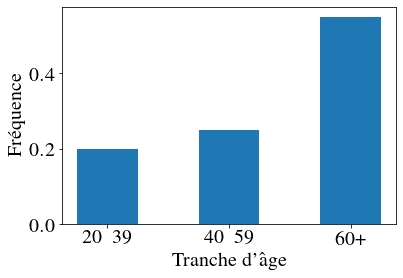
\includegraphics[width=.5\textwidth]{figures/stats/remboursement_age_bars}
	%   \caption{Diagramme en bâtons de la fréquence des tranches d'âges dans les
		%     données du tableau~\ref{tab:remboursement_data}.}
	%   \label{fig:remboursement_age_bars}
	% \end{figure}
\begin{figure}[h]
	\centering
	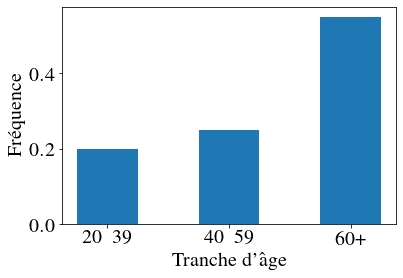
\includegraphics[width=.5\textwidth]{figures/stats/remboursement_age_bars}
	\caption{Diagramme en bâtons de la fréquence des tranches d'âges dans les
		données de remboursement.}
	\label{fig:remboursement_age_bars}
\end{figure}

Dans le cas d'une variable continue, la constitution des classes de valeurs
d'une série statistique est une étape importante. La \textbf{règle de Sturges}
propose de découper les valeurs observées en $k = \lfloor 1 + \log_2(n)\rfloor$
intervalles de même taille $\frac{\max(x_i) - \min(x_i)}{k}$. Cependant, cette
règle suppose que la variable analysée suive une distribution gaussienne ; elle
n'est pas appropriée, par exemple, si les valeurs s'étalent sur plusieurs
échelles de grandeur, auquel cas une transformation logarithmique s'imposera.

% Cela nous permet ensuite de construire une \textbf{table des fréquences} qui
% associe à chaque classe de valeurs la fréquence de cette valeur dans la
% population observée.

\begin{exemple}
	Prenons par exemple, 31 observations de la température minimale (en
	\si{\celsius}) pour la station météo de Paris-Montsouris, telles que relevées
	dans la première colonne de la table~\ref{tab:meteo_data}.
	
	Nous disposons de $n=31$ observations, qu'il s'agit, en appliquant la règle de
	Sturges, de grouper en 5 intervalles d'amplitude 2,24\si{\celsius}. La table
	des fréquences des températures minimales est donnée dans le
	tableau ci-dessous : \par % ~\ref{tab:meteo_tmin_freq}.
	% \begin{table}[h]
		\vspace*{-.25em}
		\begin{table}[H]\captionsetup{labelformat=empty} 
			\centering
			\arrayrulecolor{black!70}
			\rowcolors{2}{white}{gray!20}
			\begin{tabular}{lb{1.25cm}b{1.75cm}b{1.75cm}b{1.75cm}b{1.25cm}} \toprule[1.5pt] 
				\textbf{T min} (\si{\celsius}) & < -0,16 & -0,16 -- 2,08 & 2,08 -- 4,32 & 4,32 -- 6,56 & > 6,56 \\ 
				\textbf{Fréquence} & 0,19 & 0,19 & 0,29 & 0,10 & 0,23 \\
				\bottomrule[1.5pt]
			\end{tabular}
		\end{table}
		\vspace*{-1em}
		%   \caption{Table des fréquences des températures minimales du tableau~\ref{tab:meteo_data}.}
		%   \label{tab:meteo_tmin_freq}
		% \end{table}
\end{exemple}

Pour une variable continue, la table des fréquences peut être traduite en
\textbf{histogramme,} comme illustré sur la figure~\ref{fig:meteo_tmin_hist}.

Utiliser des fréquences plutôt que des comptes permet de comparer des
populations de tailles différentes. De plus, la distribution des fréquences
d'une série statistique de la variable $x$, représentée visuellement par un
histogramme, peut être considérée comme une approximation de la distribution de
la probabilité de cette variable dans la population.

\begin{figure}[h]
	\centering
	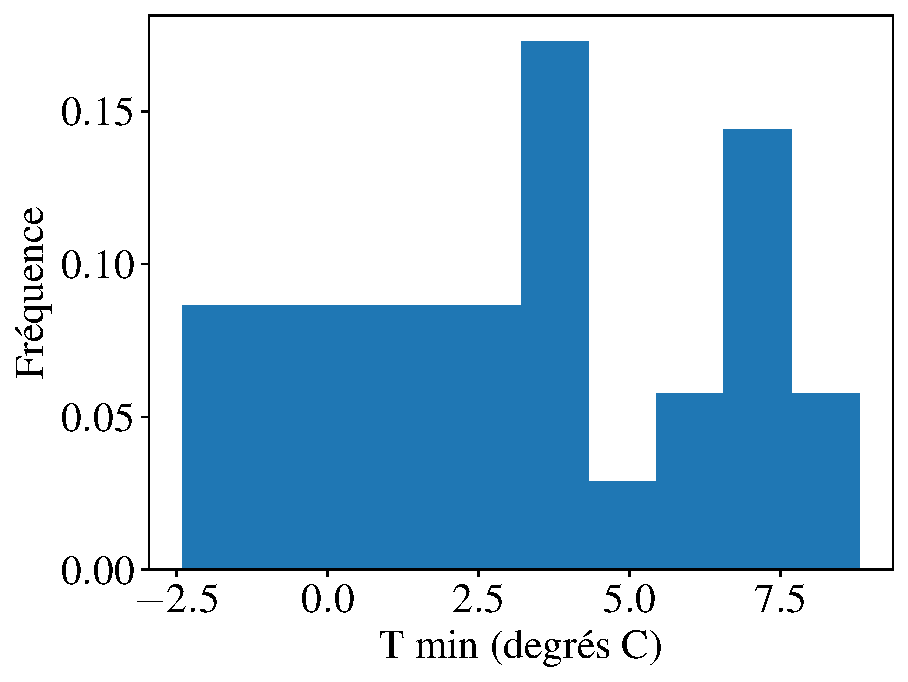
\includegraphics[width=.5\textwidth]{figures/stats/meteo_tmin_hist}
	\caption{Histogramme des températures minimales dans le
		tableau~\ref{tab:meteo_data}.}
	\label{fig:meteo_tmin_hist}
\end{figure}


\paragraph{Fréquences cumulées} 
On peut aussi choisir de représenter plutôt les \textbf{fréquences cumulées.} 

\begin{exemple}
	Pour notre série de températures minimales, la table des fréquences cumulées
	est donnée dans le tableau ci-dessous : \par % ~\ref{tab:meteo_tmin_cumul_freq}.
	% \begin{table}[h]
		\vspace*{-.25em}
		\begin{table}[H]\captionsetup{labelformat=empty} 
			\centering
			\arrayrulecolor{black!70}
			\rowcolors{2}{white}{gray!20}
			\begin{tabular}{lb{1.25cm}b{1.25cm}b{1.25cm}b{1.25cm}b{1.25cm}} \toprule[1.5pt] 
				\textbf{T min} (\si{\celsius}) & < -0,16 & < 2,08 & < 4,32 & < 6,56 & < 8,80 \\  
				\textbf{Fréquence} & 0,19 & 0,38 & 0,67 & 0,77 & 1,0 \\ \midrule[1pt]
				\textbf{T min} (\si{\celsius}) & > -2,40 & > -0,16 & > 2,08 & > 4,32 & > 6,56 \\  
				\textbf{Fréquence} & 1,0 & 0,81 & 0,62 & 0,33 & 0,23 \\ 
				\bottomrule[1.5pt]
			\end{tabular}
		\end{table}
		\vspace*{-1em}
		
		%   \caption{Table des fréquences cumulées pour les températures minimales 
			%     du tableau~\ref{tab:meteo_data}.}
		%   \label{tab:meteo_tmin_cumul_freq}
		% \end{table}
\end{exemple}

Une table des fréquences cumulées croissantes et décroissantes peut
directement être traduite en \textbf{courbes des fréquences cumulées,} comme
illustré sur la figure~\ref{fig:meteo_tmin_cumul_freq}.
\begin{figure}[h]
	\centering
	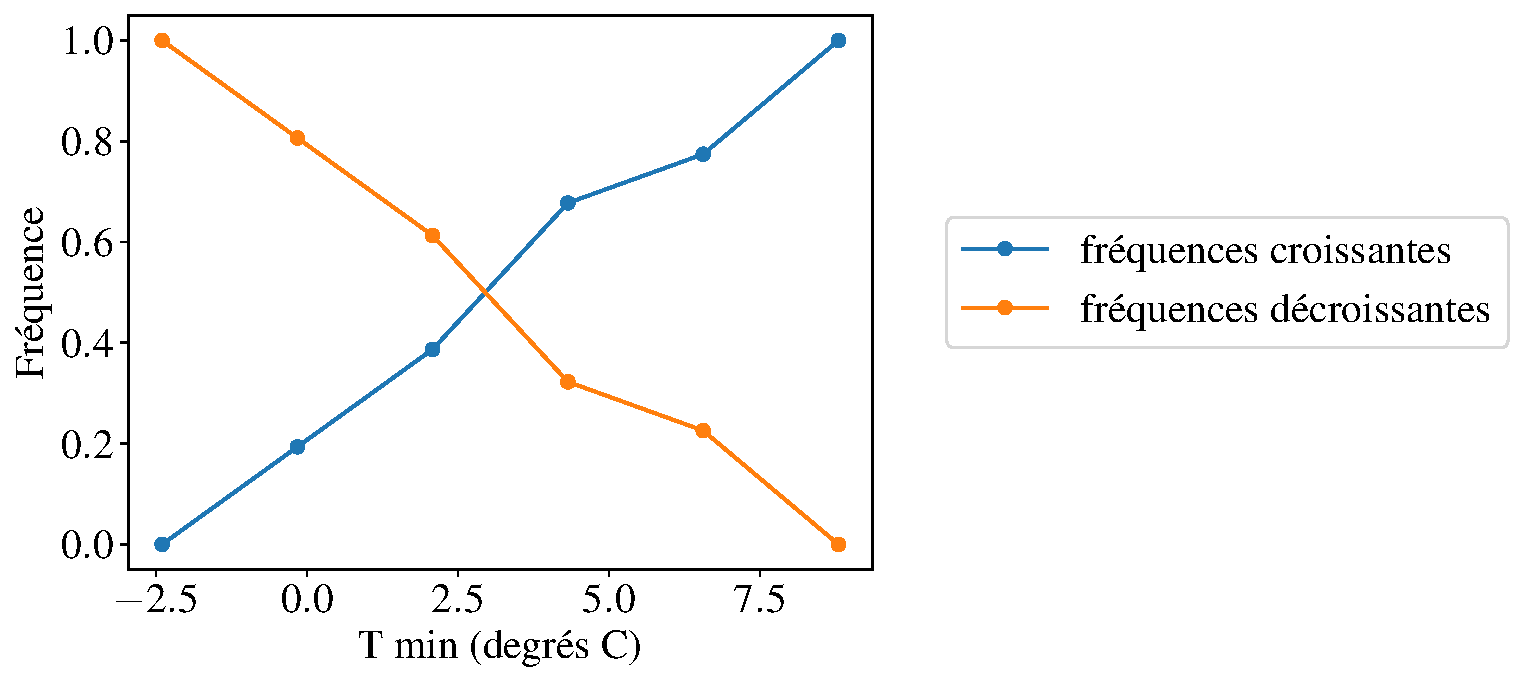
\includegraphics[width=.8\textwidth]{figures/stats/meteo_tmin_cumul_freq}
	\caption{Courbes des fréquences cumulées pour les températures minimales du
		tableau~\ref{tab:meteo_data}.}
	\label{fig:meteo_tmin_cumul_freq}
\end{figure}

\subsection{Indicateurs numériques}
Enfin, des \textbf{indicateurs numériques} permettent de compléter cette
description. On distinguera les \textbf{indicateurs de tendance centrale} qui
indiquent l'ordre de grandeur des valeurs de la série statistique et où ces
valeurs se rassemblent, des \textbf{indicateurs de dispersion} qui indiquent
l'étalement de ces valeurs.

\paragraph{Indicateurs de tendance centrale} Les indicateurs de tendance centrale comportent :
\begin{itemize}
	\item La \textbf{moyenne arithmétique} :
	\[\bar x = \frac1n \sum_{i=1}^n x_i.\]
	Elle peut être très sensible à la présence de valeurs aberrantes.
	\item La \textbf{médiane}, qui correspond à une fréquence cumulée de 50\%.
	\item Le \textbf{mode}, qui est la valeur la plus fréquente dans la série
	statistique. Il n'a réellement de sens que pour une variable discrète ;
	dans le cas d'une variable continue, on parlera plutôt, lorsque la série est
	classée, de \textbf{classe modale} qui est la classe la plus fréquente.
\end{itemize}

\begin{exemple}
	Pour notre série de températures minimales,
	\begin{itemize}
		\item la moyenne arithmétique vaut $3,2 \si{\celsius}$ ;
		\item la médiane vaut $4 \si{\celsius}$ ;
		\item la classe modale est $2,1$ -- $4,4 \si{\celsius}$.
	\end{itemize}
\end{exemple}

\paragraph{Indicateurs de dispersion} Les indicateurs de dispersion comportent : 
\begin{itemize}
	\item La \textbf{variance de la série statistique} :
	\[ \text{var}(x_1, x_2, \dots, x_n) = \frac1n \sum_{i=1}^n (x_i - \bar x)^2.\]
	\item La \textbf{variance d'échantillonnage} :
	\[ \text{var}^*(x_1, x_2, \dots, x_n) = \frac1{n-1} \sum_{i=1}^n (x_i - \bar
	x)^2.\]
	Elle est d'autant plus proche de la variance que le
	nombre d'observations est grand. Nous verrons dans la
	section~\ref{sec:unbiased_variance_estimation} qu'il s'agit d'une estimation
	\textbf{non-biaisée} de la variance de la population.
	\item L'\textbf{écart-type}, qui est la racine carrée de la variance.
	\item Le \textbf{coefficient de variation} :
	\[ \text{CV}(x_1, x_2, \dots, x_n) = \frac{\text{var}(x_1, x_2, \dots, x_n)}{\bar
		x}.\]
	Il permet d'apprécier la variabilité d'une variable
	en fonction de sa valeur moyenne, et n'a de sens que pour une variable donnée
	sur une échelle dotée d'un zéro absolu, c'est-à-dire dans laquelle une valeur
	de $2z$ peut effectivement être considérée comme deux fois plus qu'une valeur
	de $z$ (ce n'est pas le cas pour une température en degrés Celsius :
	10\si{\celsius} n'est pas « deux fois plus chaud » que 5\si{\celsius}). De
	plus, il est numériquement instable quand $\bar x$ est proche de 0.
\end{itemize}
%\pagebreak

\begin{exemple}
	La variance de notre série de températures minimales vaut $10,02 \si{\celsius^2}$,
	tandis que la variance d'échantillonage vaut $10,36 \si{\celsius^2}$. Les
	écarts-types correspondants valent tous les deux $3,2 \si{\celsius}$.  Le
	coefficient de variation n'a pas de sens en degrés Celsius.
\end{exemple}
\paragraph{Remarques}
\begin{itemize}
	\item L'écart-type d'une variable, qui s'exprime dans la même unité que la
	variable, est beaucoup plus facile à interpréter que la variance. On donne
	plus facilement un sens à $3,2 \si{\celsius}$ qu'à $10,02 \si{\celsius^2}$.
	\item L'écart-type est utilisé pour définir une erreur de mesure. Imaginons que
	l'on prenne 10 fois la même mesure, obtenant ainsi une série de 10
	mesures, de moyenne arithmétique $m$ et d'écart-type $\sigma$ ; on rapporte
	alors une valeur de $m \pm \sigma$. Cette remarque est une brève incursion
	dans le domaine de la \textit{métrologie}.
\end{itemize}

Enfin, les \textbf{quantiles} permettent aussi de déterminer la dispersion
d'une variable. Les $q$-quantiles divisent les valeurs prises par la variable
en $q$ intervalles de mêmes fréquences. Le $p$-ème $q$-quantile de
$(x_1, x_2, \dots, x_n)$ est défini comme la valeur $Q_p^q$ telle que 
\[\text{Freq}(x \leq Q_p^q) = \frac{p}{q}.\]

Lorsque $q=4,$ on parle de \textbf{quartiles.} Lorsque $q=10,$ on parle de
\textbf{déciles.}

\begin{exemple}
	Les trois quartiles de notre série de températures minimales sont
	$0,8 \si{\celsius}$, $4,0 \si{\celsius}$ et $5,6 \si{\celsius}$ : 25\% des
	valeurs observées sont inférieures à $0,8 \si{\celsius}$, 50\% sont inférieures
	à 4,0 \si{\celsius} et 75\% sont inférieures à $5,6 \si{\celsius}$. Le deuxième
	quartile correspond bien à la médiane.
\end{exemple}

Une \textbf{boîte à moustaches} (ou \textit{boxplot}) permet de résumer
visuellement ces indicateurs, comme illustré sur la
figure~\ref{fig:meteo_tmin_boxplot}. La boîte à moustaches est composée d'un
rectangle, d'une largeur arbitraire et délimité en bas par la valeur du premier
quartile et en haut par la valeur du troisième quartile ; d'une barre
horizontale au niveau de la médiane ; et de deux segments joignant chacun les
extrémités du rectangle aux valeurs les plus extrêmes. Représenter les valeurs
prises par la variable par un nuage de points superposé à ce rectangle permet
d'en faciliter l'interprétation.

\begin{figure}[h]
	\centering
	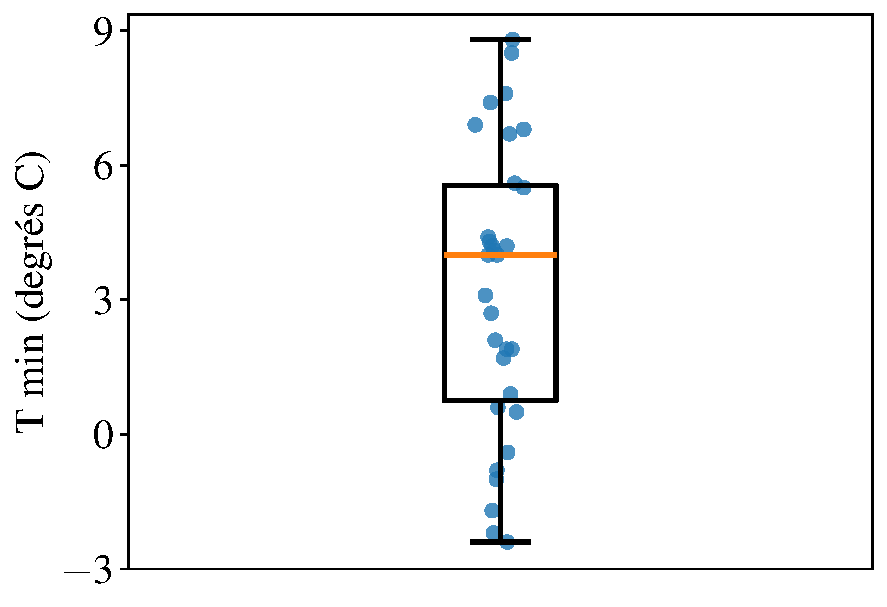
\includegraphics[width=.5\textwidth]{figures/stats/meteo_tmin_boxplot}
	\caption{Boîte à moustaches des températures minimales du
		tableau~\ref{tab:meteo_data}.}
	\label{fig:meteo_tmin_boxplot}
\end{figure}

\section{Statistique descriptive bidimensionelle}
Il s'agit ici de mettre en évidence une éventuelle \textbf{liaison,}
c'est-à-dire une variabilité simultanée, entre deux variables statistiques $x$
et $y$, observées sur $n$ individus, à travers les séries statistiques
$(x_1, x_2, \dots, x_n)$ et $(y_1, y_2, \dots, y_n).$

Cette liaison peut être causale ou non. Mettre en évidence une causalité est
délicat, et dépasse le cadre de ce cours.

Expliciter la liaison entre deux variables nous permet de comprendre :
\begin{itemize}
	\item Si une variable peut dépendre d'une autre : la température minimale
	dépend-elle de l'ensoleillement ?
	\item Si une variable peut permettre de prédire une autre : la température
	minimale permet-elle de prédire la température maximale ?
	\item Si une variable peut être remplacée par une autre : ai-je besoin de
	prendre en compte les températures minimale et maximale, ou bien
	la température moyenne suffit-elle ?
\end{itemize}

\subsection{Liaison entre deux variables quantitatives}

\paragraph{Nuage de points}
Pour visualiser la liaison entre deux variables quantitatives, on utilise
généralement un \textbf{nuage de points}. Si $x$ et $y$ sont homogènes,
c'est-à-dire exprimées dans la même unité, on utilisera la même échelle sur les
deux axes, comme sur la figure~\ref{fig:meteo_tmin_tmax}. Sinon, on préfèrera
généralement \textbf{centrer} (retrancher la moyenne) et \textbf{réduire} (diviser par l'écart-type) les variables au préalable, comme sur la
figure~\ref{fig:meteo_tmin_vent} : 
\[
\forall\,i\in \llbracket 1, n \rrbracket \quad x_i \leftarrow \frac{x_i - \bar x}{\sigma_x}, \qquad \text{avec} \quad \bar x = \frac{1}{n} \sum_{i=1}^n x_i \quad
\text{et} \quad \sigma_x = \sqrt{\frac{1}{n} \sum_{i=1}^n(x_i - \bar x)^2}.
\]

\begin{figure}[h]
	\centering
	\begin{subfigure}[t]{0.49\textwidth}
		\centering
		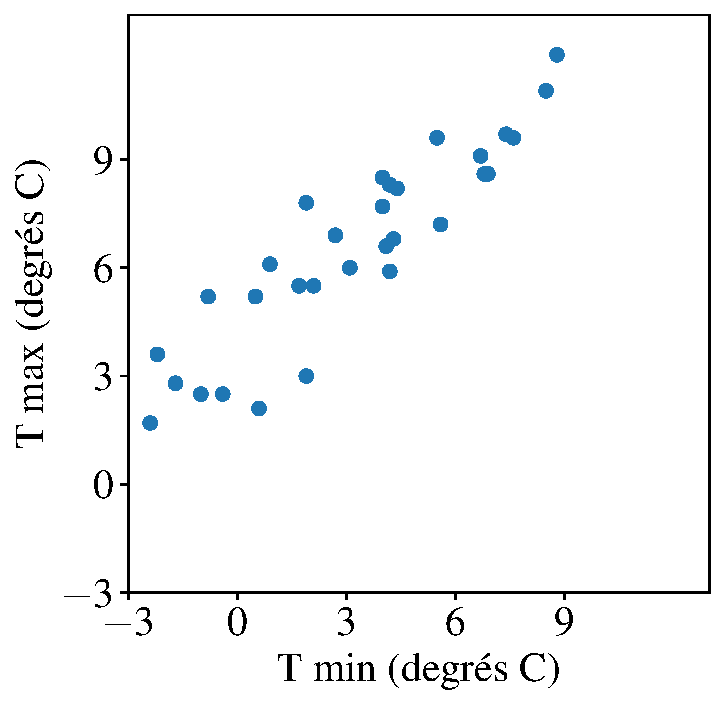
\includegraphics[width=.7\textwidth]{figures/stats/meteo_tmin_tmax}
		\caption{Températures maximales vs minimales.}
		\label{fig:meteo_tmin_tmax}
	\end{subfigure} \hfill
	\begin{subfigure}[t]{0.49\textwidth}
		\centering
		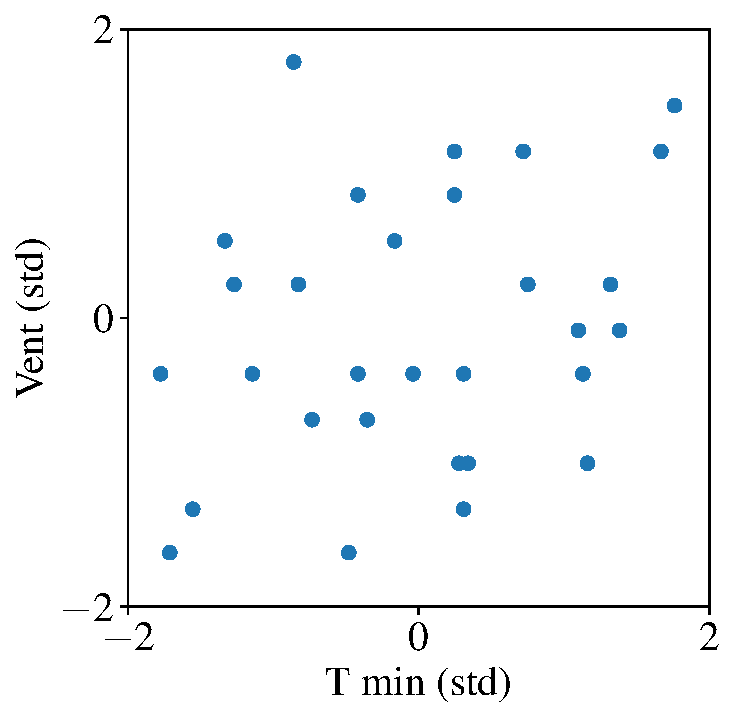
\includegraphics[width=.7\textwidth]{figures/stats/meteo_tmin_vent}
		\caption{Vent vs températures minimales.}
		\label{fig:meteo_tmin_vent}
	\end{subfigure}
	\caption{Nuages de points pour des paires de variables du
		tableau~\ref{tab:meteo_data}.}
\end{figure}


\paragraph{Indicateurs de liaison entre deux variables quantitatives}
Pour quantifier la liaison entre deux variables quantitatives, on utilise
principalement :
\begin{itemize}
	\item \textbf{La covariance} :
	\[\text{cov}(x, y) = \frac1n \sum_{i=1}^n (x_i - \bar x) (y_i - \bar y).\]
	\item \textbf{Le coefficient de corrélation de Pearson,} qui est égal à la
	covariance entre les variables centrées réduites, et compris entre $-1$ et $1$ :
	\[r(x, y) = \frac1n \frac{\sum_{i=1}^n (x_i - \bar x) (y_i - \bar y)}{\sigma_x \sigma_y}.\]
\end{itemize}

À noter que la covariance et le coefficient de corrélation de Pearson mesurent
des liaisons \textit{linéaires} entre deux variables. Une corrélation de
Pearson proche de 1 ou de -1 indique une relation linéaire ; une corrélation de
Pearson proche de 0 indique une absence de corrélation. D'autres mesures, comme
l'information mutuelle (hors cadre de ce cours), permettent de mesurer des
liaisons \textit{non-linéaires}. 

\begin{exemple}
	Pour les données du tableau~\ref{tab:meteo_data}, la covariance entre la
	température minimale et la température maximale vaut $7,69 \si{\celsius^2}$ ;
	leur corrélation de Pearson vaut 0,91. La corrélation de Pearson entre vent
	et température minimale vaut 0,28. La figure~\ref{fig:pearson} illustre le
	rapport entre corrélation de Pearson et nuage de points.
\end{exemple}
\begin{figure}[h]
	\centering
	\begin{subfigure}[t]{0.24\textwidth}
		\centering
		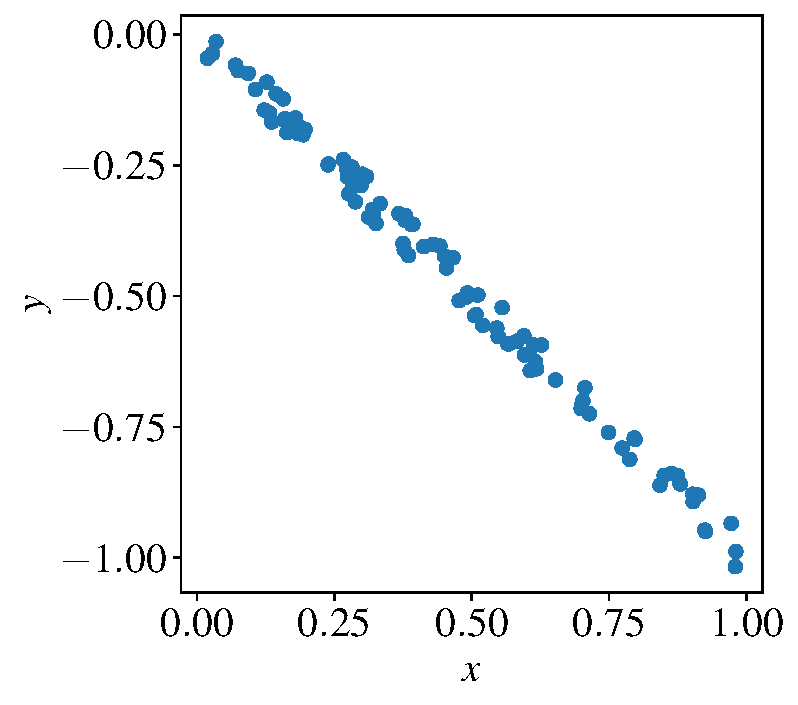
\includegraphics[width=\textwidth]{figures/stats/pearson_3}
		\caption{r(x, y) = -1,00.}
	\end{subfigure} \hfill
	\begin{subfigure}[t]{0.24\textwidth}
		\centering
		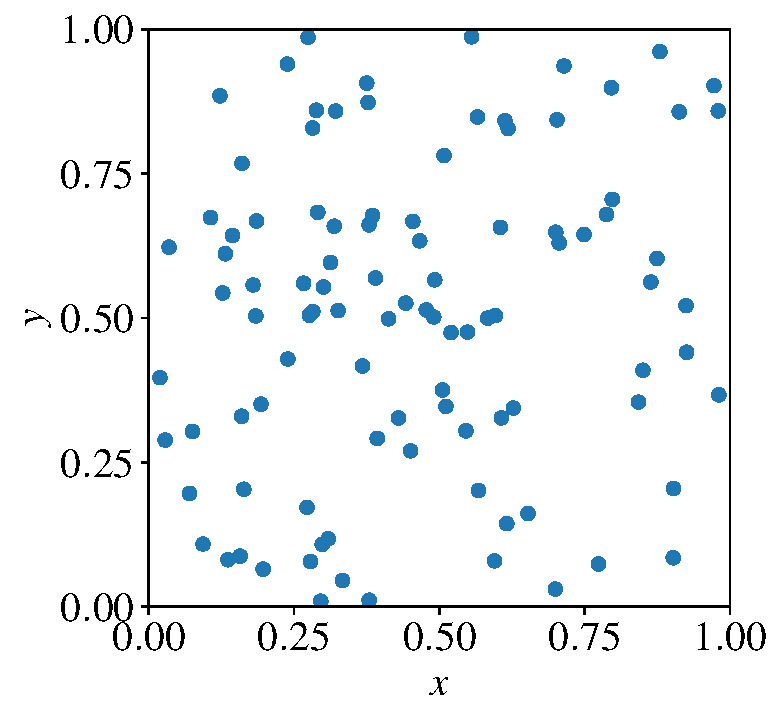
\includegraphics[width=\textwidth]{figures/stats/pearson_0}
		\caption{r(x, y) = 0,03.}
	\end{subfigure} \hfill
	\begin{subfigure}[t]{0.24\textwidth}
		\centering
		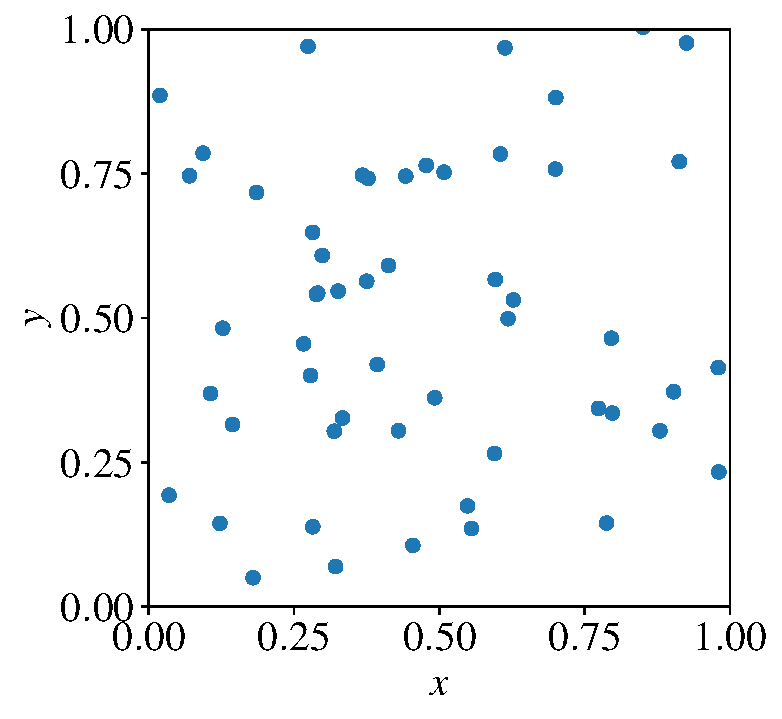
\includegraphics[width=\textwidth]{figures/stats/pearson_2}
		\caption{r(x, y) = 0,53.}
	\end{subfigure} \hfill
	\begin{subfigure}[t]{0.24\textwidth}
		\centering
		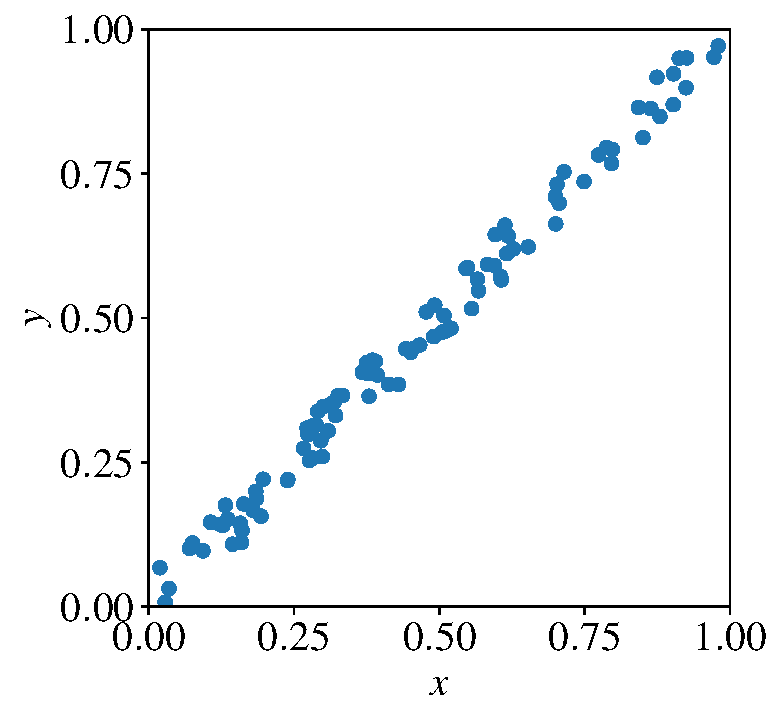
\includegraphics[width=\textwidth]{figures/stats/pearson_1}
		\caption{r(x, y) = 1,00.}
	\end{subfigure} \hfill
	\caption{Nuages de points entre deux variables simulées et leur corrélation de Pearson.}
	\label{fig:pearson}
\end{figure}

\paragraph{Indicateurs de liaison entre une variable qualitative et une variable quantitative}
Pour étudier la liaison entre une variable qualitative $x$, ayant $K$ modalités dans la série statistique $(x_1, x_2, \dots, x_n),$ et une
variable quantitative $y,$ on considère que la variable $x$ permet de définir
$K$ sous-populations. Il s'agit alors d'évaluer s'il existe des différences,
pour la variable $y$, entre ces sous-populations.

Visuellement, on utilisera une série de boîtes à moustaches, comme illustré sur
la figure~\ref{fig:remboursement_rembourses_age}.

% \begin{figure}[h]
	%   \centering
	%   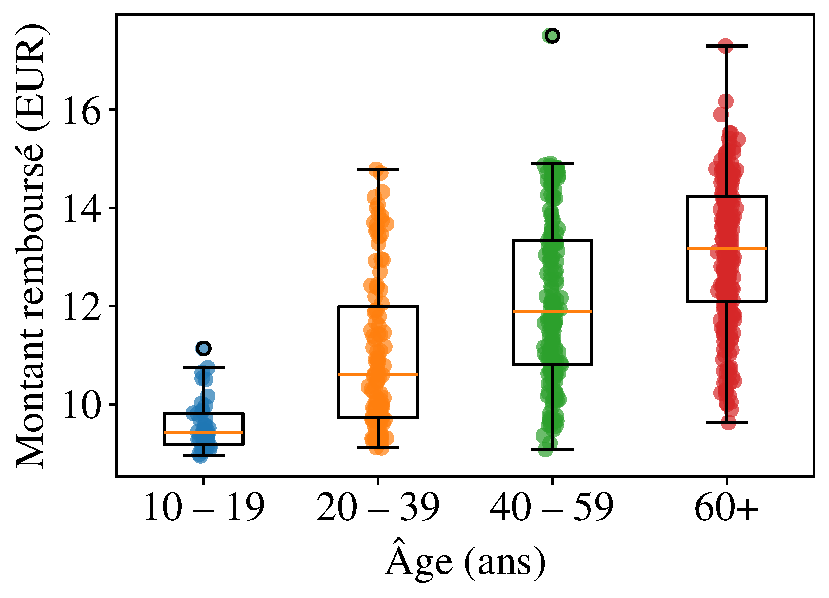
\includegraphics[width=.5\textwidth]{figures/stats/remboursement_rembourses_age}
	%   \caption{Montants remboursés par acte, par tranche d'âge, pour les données du
		%     tableau~\ref{tab:remboursement_data}.}
	%   \label{fig:remboursement_rembourses_age}
	% \end{figure}
\begin{figure}[h]
	\centering
	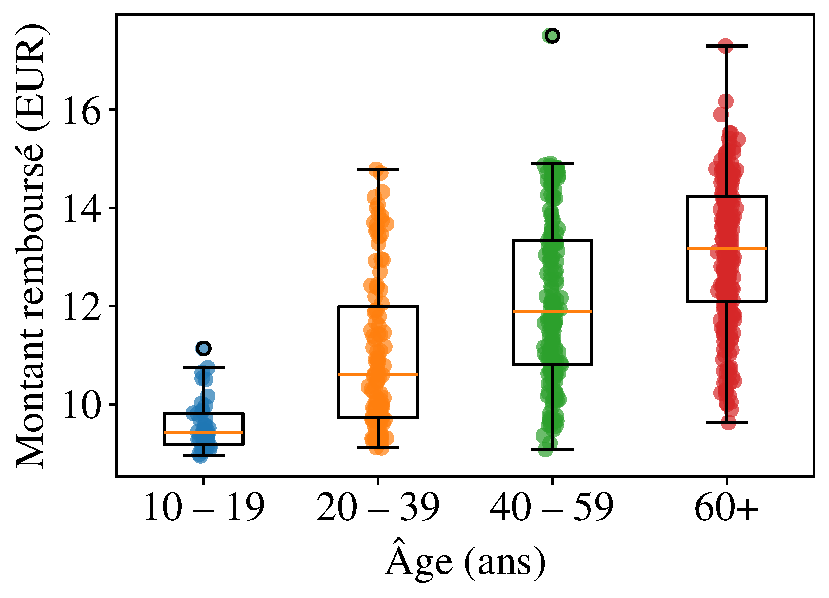
\includegraphics[width=.5\textwidth]{figures/stats/remboursement_rembourses_age}
	\caption{Montants remboursés par acte, par tranche d'âge, pour les données de
		remboursement.}
	\label{fig:remboursement_rembourses_age}
\end{figure}

La \textbf{variance expliquée} par $x$ de $y$ est la moyenne des carrés des écarts
entre la moyenne de $y$ dans chaque sous-population et la moyenne de $y$ dans
toute la population, pondérée par la taille des sous-populations :
\[
\sigma_E^2 = \frac1n \sum_{k=1}^K n_k (\bar{y}_k - \bar{y})^2,
\]
où $n_k$ est le nombre d'individus dans la sous-population $k$, $\bar{y}_k$ la moyenne de $y$ dans cette sous-population et $\bar{y}$
la moyenne de $y$ dans la population totale.

La \textbf{variance résiduelle} est la moyenne des variances des
sous-populations, pondérées par leur taille :
\[
\sigma_R^2 = \frac1n \sum_{k=1}^K n_k \sigma_k^2, 
\]
où $\sigma_k^2$
est la variance de $y$ dans la sous-population $k$.


On peut montrer que $\sigma_y^2 = \sigma_R^2 + \sigma_E^2.$

Le \textbf{rapport de corrélation} est la part de variation de $y$ expliquée
par $x$. Compris entre 0 et 1, il est d'autant plus élevé que la liaison entre
les deux variables est forte :
\[
e^2  = \frac{\sigma_E^2}{\sigma_y^2}.
\]
\begin{exemple}
	% Pour les montants remboursés par acte du tableau~\ref{tab:remboursement_data},
	% la variance de ces montants est de 3,65, tandis que la variance expliquée par
	% l'âge est de 1,37 (en euros au carré), ce qui donne un rapport de corrélation
	% de 0,38.
	Pour les montants remboursés par acte de nos données de remboursement, la
	variance de ces montants est de $3,30$\texteuro$^2$, tandis que la variance
	expliquée par l'âge est de $1,09$\texteuro$^2$, ce qui donne un rapport de
	corrélation de $0,33.$ 
\end{exemple}

\paragraph{Indicateurs de liaison entre deux variables qualitatives}
Pour étudier la liaison entre une variable qualitative $x$ ayant $K$ modalités $v_1,\dots,v_K$ dans la série statistique $(x_1, x_2, \dots, x_n),$ et une
variable qualitative $y$ ayant $L$ modalités $w_1,\dots,w_L$ dans la série statistique
$(y_1, y_2, \dots, y_n),$ on utilise généralement une \textbf{table de
	contingence} de taille $K \times L.$ Il s'agit de compter combien d'individus présentent chacune des modalités de $x$ et de $y$ : l'élément $n_{k\ell}$ à l'intersection de la $k^{\text{ème}}$ ligne et de la $\ell^{\text{ème}}$ colonne de la table de contingence correspond au le nombre d'individus pour lesquels $x = v_k$ et $y = w_\ell$.

Si l'on appelle $n_{k\boldsymbol{.}} = \sum_{\ell=1}^L n_{k\ell}$ le nombre d'individus ayant la modalité
$v_k$ pour $x$ et $n_{\boldsymbol{.}\ell} = \sum_{k=1}^K n_{k\ell}$ le nombre d'individus ayant la modalité $w_\ell$ pour $y$,
alors l'absence de liaison entre $x$ et $y$ se traduit par l'égalité :
\[
\frac{n_{k\ell}}{n} = \frac{n_{k\boldsymbol{.}}}{n}
\frac{n_{\boldsymbol{.}\ell}}{n} \quad \text{pour tout} \quad
1 \leq k \leq K,\; 1 \leq \ell \leq L.
\]
L'écart entre les valeurs prises de part et d'autre de cette égalité se mesure
grâce à la \textbf{distance du chi2}, définie par 
\[
d_{\chi^2} = \sum_{k=1}^K \sum_{\ell=1}^L  \dfrac{\left( n_{k\ell} - 
	\frac{n_{k\boldsymbol{.}}n_{\boldsymbol{.}\ell}}{n} \right)^2}{\frac{n_{k\boldsymbol{.}}n_{\boldsymbol{.}\ell}}{n}}.
\]

\begin{exemple}
	La table de contingence pour les variables « âge » et « région » des données
	de remboursement est donnée dans le
	tableau~\ref{tab:remboursement_age_region}. La distance du chi2 pour cette
	table de contingence est de 11,21, ce qui suggère une dépendance entre les
	variables « âge » et « région » dans les données.
\end{exemple}


\begin{table}[h]
	\centering
	\arrayrulecolor{black!70}
	\rowcolors{3}{gray!20}{white}
	\begin{tabular}[h]{ccccccccccccccc}
		\cmidrule[1.5pt]{3-15}
		& & \multicolumn{13}{c}{\textbf{Région}} \\ \cmidrule{3-15}
		& & 5 & 11 & 24 & 27 & 28 & 32 & 44 & 52 & 53 & 75 & 76 & 84 & 93 \\ \midrule[1pt]
		\cellcolor{white}& \multicolumn{1}{|c!{\color{black!70}\vrule width 1pt}}{0--19} & 3 & 5 & 3 & 3 & 3 & 3 & 4 & 3 & 2 & 3 & 3 & 4 & 4 \\ 
		\cellcolor{white}& \multicolumn{1}{|c!{\color{black!70}\vrule width 1pt}}{20--39} & 8 & 18 & 4 & 7 & 4 & 9 & 11 & 6 & 4 & 7 & 8 & 10 & 11 \\ 
		\cellcolor{white}& \multicolumn{1}{|c!{\color{black!70}\vrule width 1pt}}{40--59} & 11 & 26 & 11 & 13 & 13 & 16 & 15 & 10 & 8 & 12 & 17 & 15 & 19 \\ 
		\cellcolor{white}\raisebox{20pt}[0pt][0pt]{\rotatebox[origin=c]{0}{\parbox{1cm}{\centering\textbf{Âge}}}} & \multicolumn{1}{|c!{\color{black!70}\vrule width 1pt}}{$>$ 60} & 15 & 31 & 18 & 16 & 21 & 21 & 22 & 12 & 12 & 19 & 24 & 23 & 26 \\
		\bottomrule[1.5pt]
	\end{tabular}
	\caption{Table de contingence pour l'âge et la région des données 
		de remboursement.}
	\label{tab:remboursement_age_region}
\end{table}



% Nous verrons dans la PC1 comment transformer cette distance en
% un test statistique de dépendance.

% \begin{table}[h]
	%   \centering
	%   \begin{tabular}[h]{|c|c|c|c|c|c|c|c|c|c|c|}
		%     \hline
		%     & \multicolumn{10}{|c|}{Région} \\ \hline
		%     {Âge} & 5 & 11 & 24 & 27 & 32 & 44 & 75 & 76 & 84 & 93 \\ \hline
		%     20--39 & 1 & 1 & 0 & 0 & 2 & 0 & 0 & 0 & 0 & 0 \\ \hline
		%     40--59 & 0 & 1 & 0 & 0 & 1 & 1 & 0 & 1 & 1 & 0 \\ \hline
		%     $>$ 60 & 1 & 1 & 1 & 1 & 2 & 1 & 1 & 2 & 0 & 1 \\ \hline
		%   \end{tabular}
	%   \caption{Table de contingence pour l'âge et la région des données 
		%     du tableau~\ref{tab:remboursement_data}.}
	%   \label{tab:remboursement_age_region}
	% \end{table}

La table de contingence peut être visualisée grâce à deux \textbf{diagrammes en
	barres empilées} : on peut choisir de visualiser, pour chaque modalité de $x$, la
proportion relative des modalités de $y$, ou inversement, pour chaque modalité de $y$,
la proportion relative des modalités de $x$. Ces deux choix sont illustrés sur les
figures~\ref{fig:remboursement_age_region_lines}
et~\ref{fig:remboursement_age_region_cols} respectivement.

\begin{figure}[H]
	\centering
	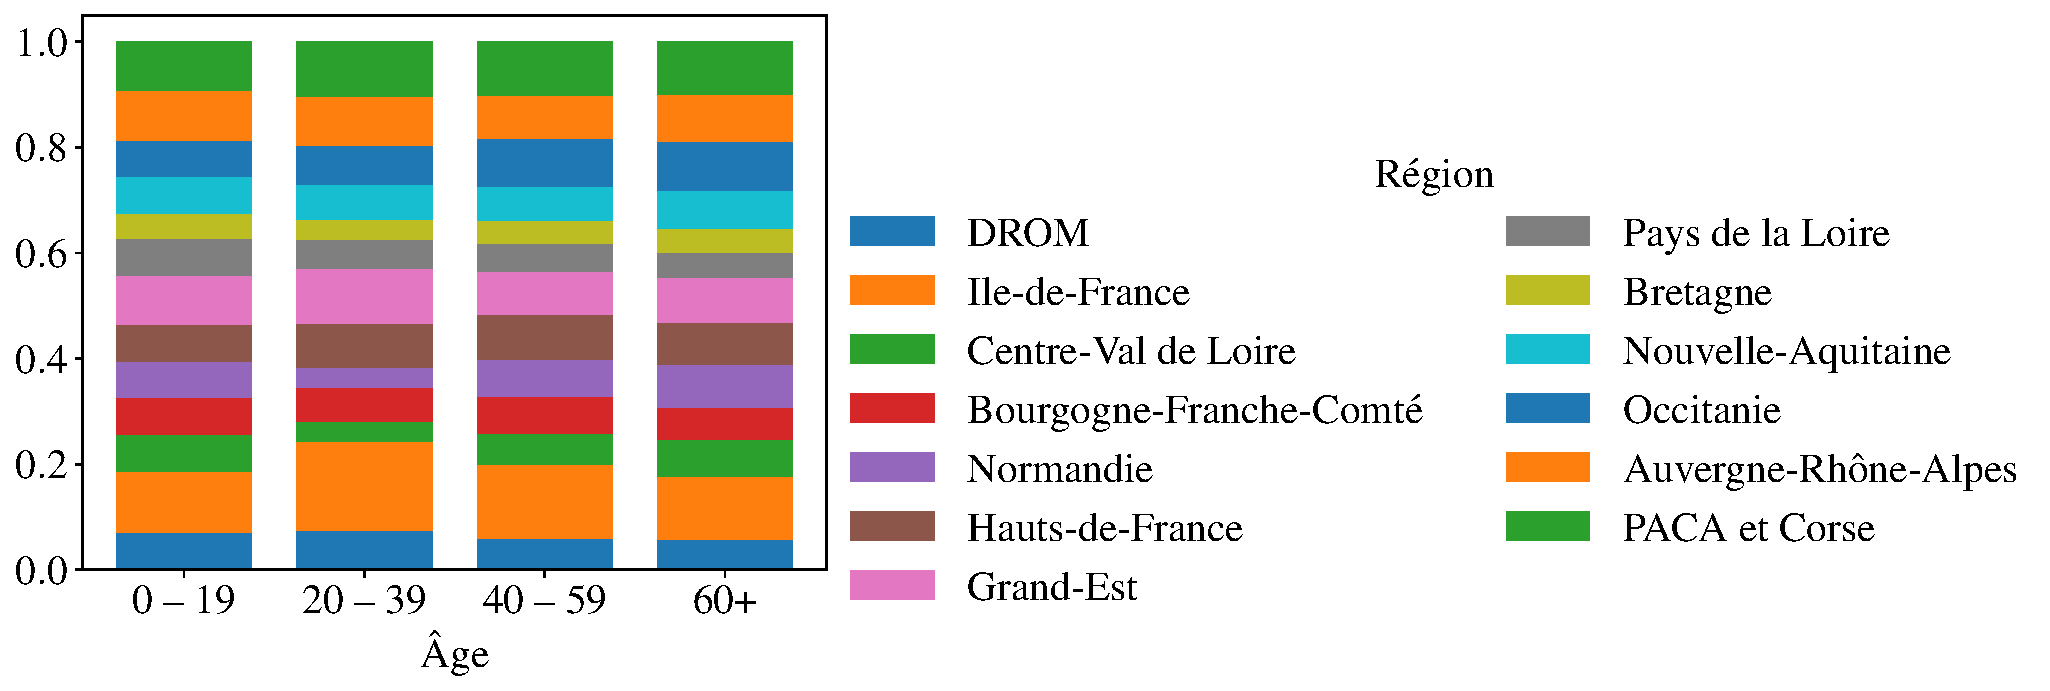
\includegraphics[width=\textwidth]{figures/stats/remboursement_age_region_lines}
	\caption{Diagramme en barres représentant, pour chaque tranche d'âges, la
		proportion relative d'individus de chaque région dans la table de
		contingence du tableau~\ref{tab:remboursement_age_region}.}
	\label{fig:remboursement_age_region_lines}
\end{figure}

\begin{figure}[H]
	\centering
	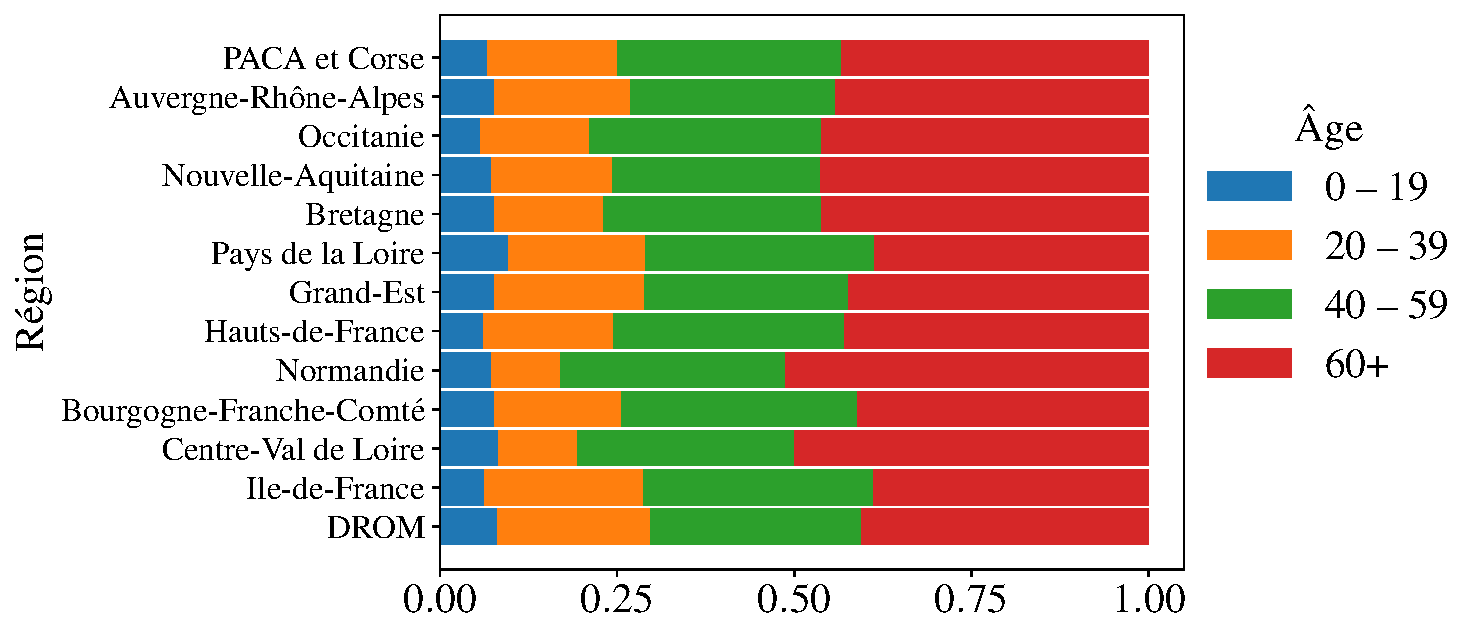
\includegraphics[width=\textwidth]{figures/stats/remboursement_age_region_cols}
	\caption{Diagramme en barres représentant, pour chaque région, la proportion
		relative d'individus de chaque tranche d'âge dans la table de contingence du
		tableau~\ref{tab:remboursement_age_region}.}
	\label{fig:remboursement_age_region_cols}
\end{figure}

%\clearpage
%-*- coding: utf-8 -*-
\section{QCM}
\paragraph{Question 1.} On s'intéresse aux hospitalisations pour une certaine
maladie. Comment visualiser la liaison entre la durée du séjour à l'hôpital et
l'âge des patients, la première étant donnée en nombre de jours et le second
par tranches ?
\begin{itemize}
	\item[$\square$] Par un nuage de points 
	\item[$\square$] Par un diagramme en barres
	\item[$\square$] Par une série de boîtes à moustaches
\end{itemize}

\paragraph{Question 2.} L'image ci-dessous représente un nuage de points entre
le diamètre de fleurs et la hauteur de leur tige. Leur coefficient de
corrélation de Pearson est plutôt proche de...
\begin{itemize}
	\item[$\square$] $- 0,35$
	\item[$\square$] $+ 0,35$
	\item[$\square$] $- 0,85$
	\item[$\square$] $+ 0,85$
	\item[$\square$] $- 0,95$
	\item[$\square$] $+ 0,95$
	\item[$\square$] $- 0,50$
	\item[$\square$] $+ 0,50$
\end{itemize}

\vspace{-13em}
\begin{center}
	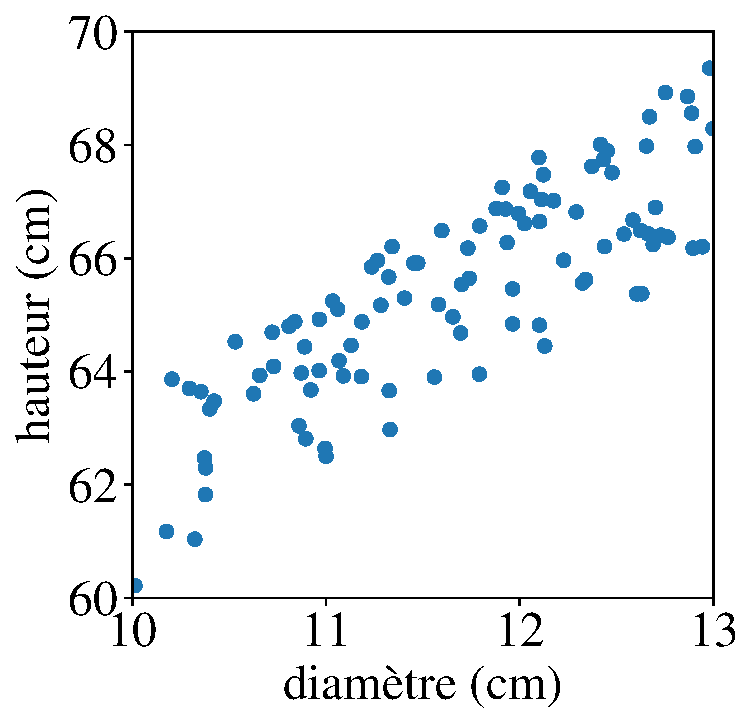
\includegraphics[width=0.35\textwidth]{figures/pearson_example}
\end{center}



\section*{Solution}
{%
	\noindent
	\rotatebox[origin=c]{180}{%
		\noindent
		\begin{minipage}[t]{\linewidth}
			\paragraph{Question 1.} Une série de boîtes à moustaches est plus appropriée
			pour visualiser la relation entre une variable quantitative (durée du séjour)
			et une variable qualitative (âge par
			tranches). Cf. figure~\ref{fig:remboursement_rembourses_age}.\newline
			
			\paragraph{Question 2.} $r \approx 0,85.$ On peut voir à la « pente » que la
			corrélation est positive. La situation est intermédiaire entre celle des
			figures 2.6(\textsc{C}) $(r=0,50)$ et 2.6(\textsc{D}) $(r=1,00)$. Une
			corrélation de $0,95$ serait plus proche de la figure~\ref{fig:pearson}(\textsc{D}) que de
			celle donnée ci-dessus. Remarquez ici que les données ne sont pas homogènes, au
			sens où elles ont des échelles de valeurs différentes, contrairement à ce qui
			est représenté sur la figure~\ref{fig:pearson} ; cela ne change pas l'interprétation de la
			corrélation.
		\end{minipage}%
	}%
	
	
	%%% Local Variables:
	%%% mode: latex
	%%% TeX-master: "../../sdd_2025_poly"
	%%% End:



%%% Local Variables:
%%% mode: latex
%%% TeX-master: "../sdd_2025_poly"
%%% End: